\documentclass[UTF8, a4paper, 11pt]{article}
\usepackage{diagbox}
\usepackage{subfigure}
\usepackage[UTF8, scheme=plain]{ctex}
\usepackage{fontspec}
\usepackage{float}
\usepackage{amsmath}
\newtheorem{myDef}{Definition}
\usepackage{graphicx}
\usepackage{geometry}
\usepackage{listings}
\usepackage{xcolor}
\usepackage{caption}
\geometry{scale=0.8}
\linespread{1.5}
\usepackage{hyperref}
\usepackage{color}
\usepackage{fontspec}
\usepackage{enumitem}
\usepackage[linesnumbered,boxed]{algorithm2e}    
\usepackage{xeCJK}
\usepackage{indentfirst} 
\graphicspath{{Pics/}} 	% 在于.tex同级的目录下创建名为pic的文件夹,存放图片


\setlength{\parindent}{2em}

\lstset{
    language={python},
    frame=shadowbox,
    breaklines=true,
    numbers=left,
    backgroundcolor=\color[RGB]{245,245,244},
    rulesepcolor=\color{red!20!green!20!blue!20},
    numberstyle={\color[RGB]{0,192,192}\tiny},
    basicstyle=\footnotesize \fontspec{Source Code Pro}
}
\setenumerate[1]{itemsep=0pt,partopsep=0pt,parsep=\parskip,topsep=0pt}
\setitemize[1]{itemsep=0pt,partopsep=0pt,parsep=\parskip,topsep=0pt}
\setdescription{itemsep=0pt,partopsep=0pt,parsep=\parskip,topsep=0pt}


\title{	
\normalfont \normalsize
\textsc{School of Data and Computer Science, Sun Yat-sen University} \\ [25pt] %textsc small capital letters
\rule{\textwidth}{0.5pt} \\[0.4cm] % Thin top horizontal rule
\huge 数电实验9\\ % The assignment title
\rule{\textwidth}{2pt} \\[0.5cm] % Thick bottom horizontal rule
\author{18308045 谷正阳}
\date{\normalsize\today}
}

\begin{document}
\maketitle
\tableofcontents
\newpage
\section{仿真实验}
\subsection{J-K触发器动态测试}
\subsubsection{电路图}
\begin{figure}[H]
    \centering
    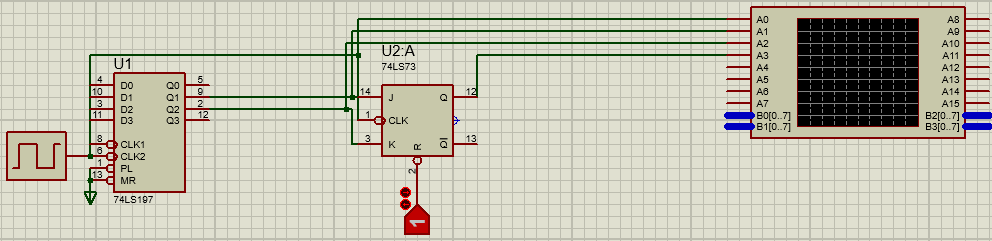
\includegraphics[width=0.8\textwidth]{ex9.1电路图.png}
\end{figure}
本次实验有点失误,并未按照实验十中的要求将10kHz接反相器再接74LS197的CP1,但是由于74LS197有延迟,给出的信号慢于CLK,因而只要看CLK翻转前一个周期的74LS197输出信号即可。
\subsubsection{波形图}
\begin{figure}[H]
    \centering
    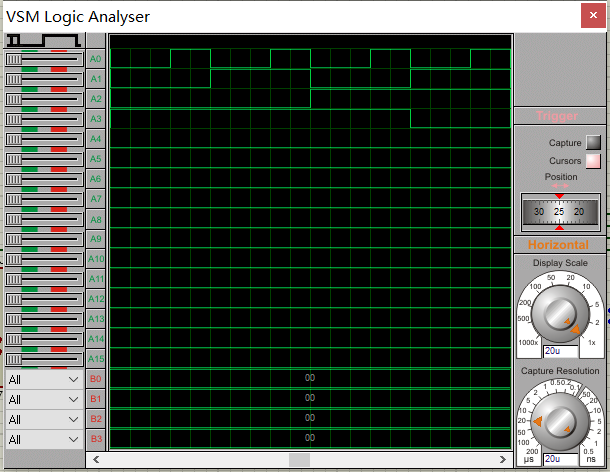
\includegraphics[width=0.8\textwidth]{ex9.1波形图.png}
\end{figure}
图中:下降沿有效,J=K=0保持,J=1,K=0置位,J=0,K=1清零,J=1,K=1翻转。
\subsection{D触发器动态测试}
\subsubsection{电路图}
\begin{figure}[H]
    \centering
    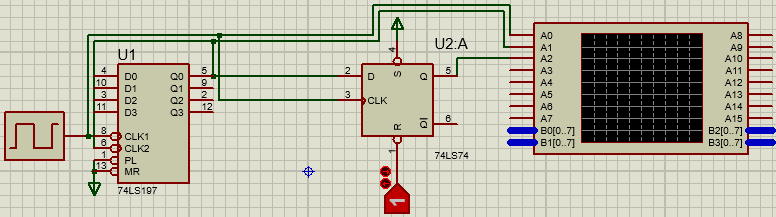
\includegraphics[width=0.8\textwidth]{ex9.2电路图.png}
\end{figure}
\subsubsection{波形图}
\begin{figure}[H]
    \centering
    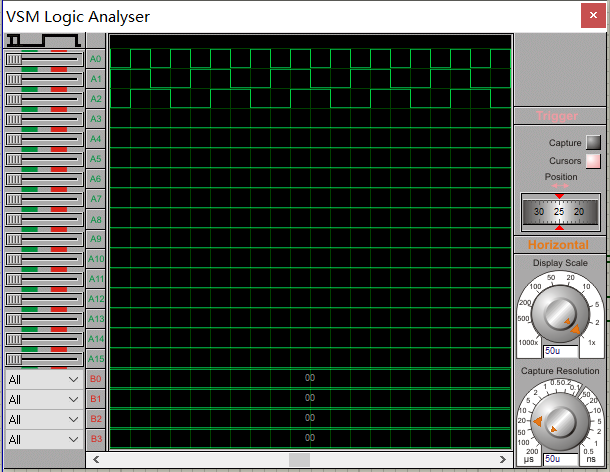
\includegraphics[width=0.8\textwidth]{ex9.2波形图.png}
\end{figure}
图中:上升沿有效,D=0清零,D=1置位。
\subsection{J-K触发器实现D触发器}
\subsubsection{电路图}
\begin{figure}[H]
    \centering
    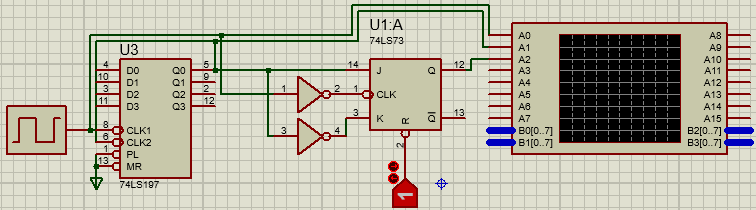
\includegraphics[width=0.8\textwidth]{ex9.3电路图.png}
\end{figure}
将J和K'相连,视为D,CLK处接非门使其变成上升沿有效。
\subsubsection{波形图}
\begin{figure}[H]
    \centering
    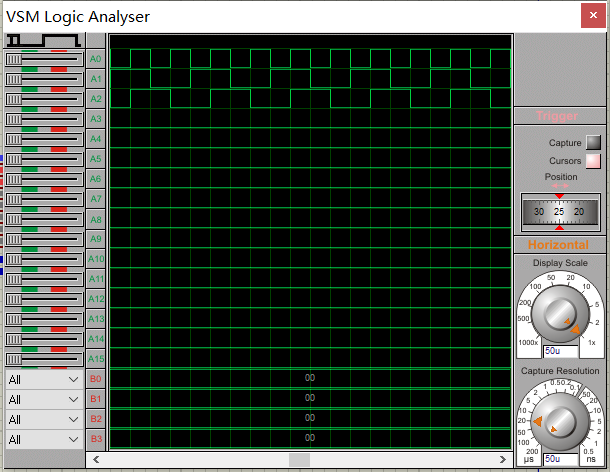
\includegraphics[width=0.8\textwidth]{ex9.3波形图.png}
\end{figure}
\subsection{J-K触发器实现T触发器}
\subsubsection{电路图}
\begin{figure}[H]
    \centering
    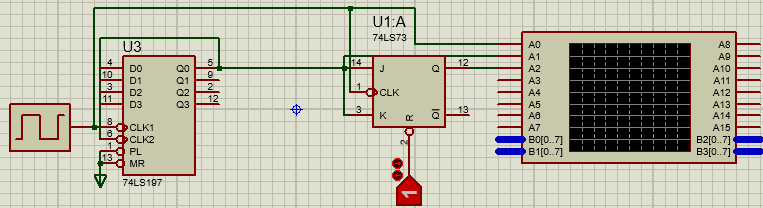
\includegraphics[width=0.8\textwidth]{ex9.4电路图.png}
\end{figure}
将J和K相连,视为T。
\subsubsection{波形图}
\begin{figure}[H]
    \centering
    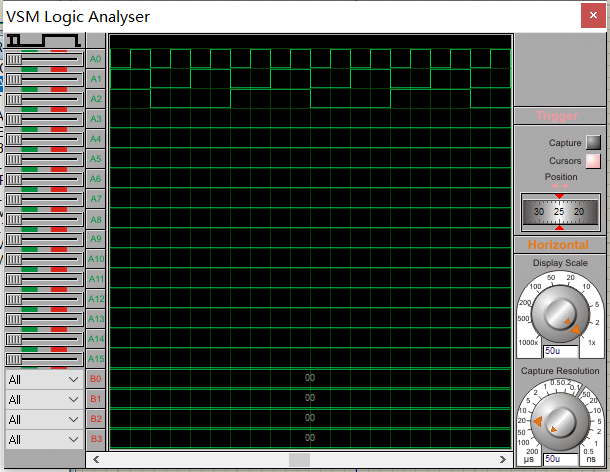
\includegraphics[width=0.8\textwidth]{ex9.4波形图.png}
\end{figure}
图中:初始化为0,下降沿有效,T=0保持,T=1翻转。
\subsection{防抖动电路}
\subsubsection{电路图}
\begin{figure}[H]
    \centering
    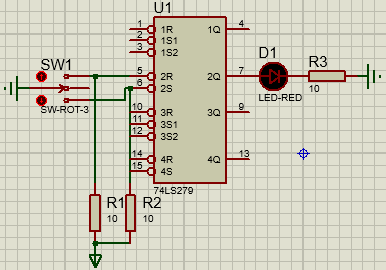
\includegraphics[width=0.8\textwidth]{ex9.5电路图.png}
\end{figure}
单刀三掷开关模仿抖动,中间表示抖动状态。
\subsubsection{静态实验}
\begin{figure}[H]
    \centering
    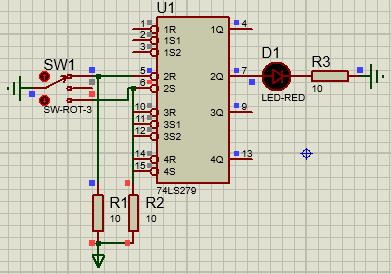
\includegraphics[width=0.8\textwidth]{ex9.5.1.png}
\end{figure}
\begin{figure}[H]
    \centering
    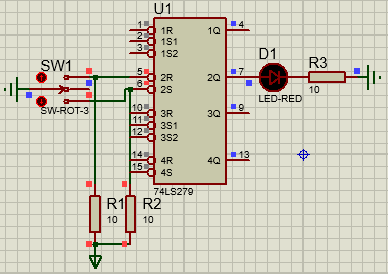
\includegraphics[width=0.8\textwidth]{ex9.5.2.png}
\end{figure}
\begin{figure}[H]
    \centering
    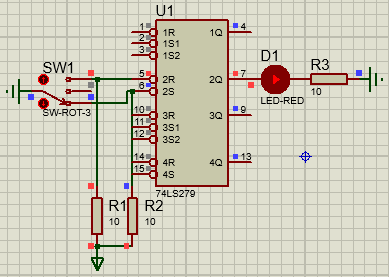
\includegraphics[width=0.8\textwidth]{ex9.5.3.png}
\end{figure}
\begin{figure}[H]
    \centering
    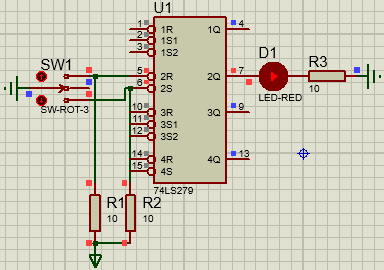
\includegraphics[width=0.8\textwidth]{ex9.5.4.png}
\end{figure}
抖动即开关接中间时,仍保持之前的状态。
\subsection{SR触发器实现}
\subsubsection{电路图}
\begin{figure}[H]
    \centering
    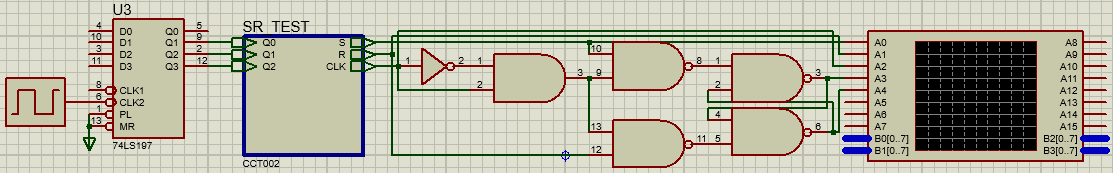
\includegraphics[width=0.8\textwidth]{ex9.6电路图.png}
\end{figure}
\begin{figure}[H]
    \centering
    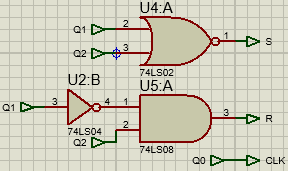
\includegraphics[width=0.8\textwidth]{ex9.6子电路图.png}
\end{figure}
子电路用于生成SR=10,00,01,00的信号,便于测试。
\subsubsection{波形图}
\begin{figure}[H]
    \centering
    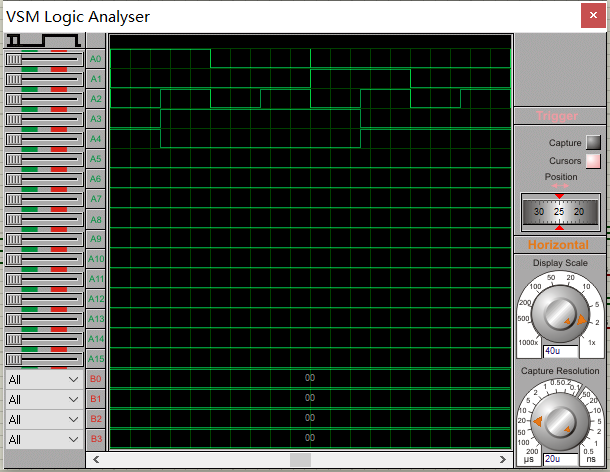
\includegraphics[width=0.8\textwidth]{ex9.6波形图.png}
\end{figure}
图中:分别为S,R,CLK,Q,Q',上升沿有效,S=1,R=0时置位,S=R=0时保持,S=0,R=1时清零,S=R=0时保持。
\subsection{D触发器实现}
\subsubsection{电路图}
\begin{figure}[H]
    \centering
    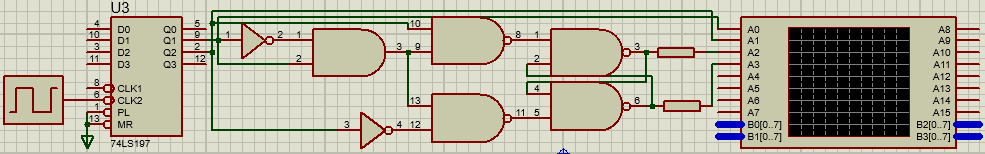
\includegraphics[width=0.8\textwidth]{ex9.7电路图.png}
\end{figure}
\subsubsection{波形图}
\begin{figure}[H]
    \centering
    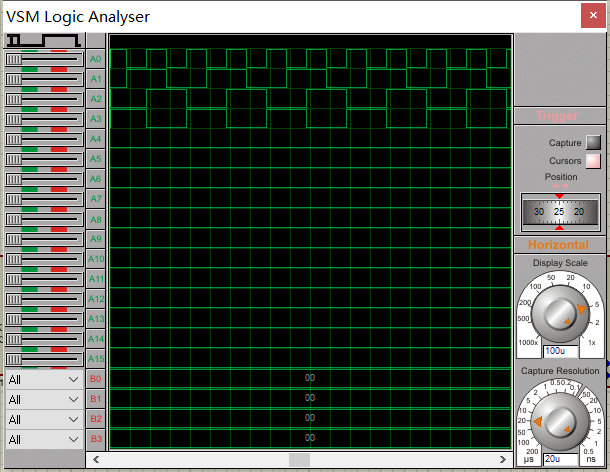
\includegraphics[width=0.8\textwidth]{ex9.7波形图.png}
\end{figure}
图中:分别为CLK,D,Q,Q',上升沿有效,D=0时清零,D=1时置位。
\section{J-K触发器实现}
\subsection{电路图}
\begin{figure}[H]
    \centering
    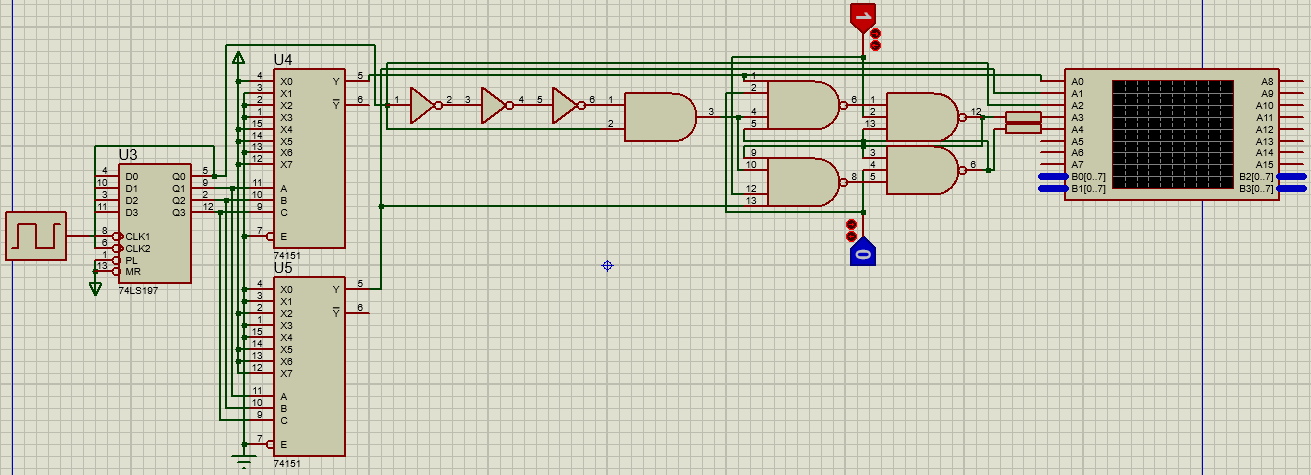
\includegraphics[width=0.8\textwidth]{ex9.8电路图.png}
\end{figure}
上面是PRE',下面是CLR',左边两个38译码器用于产生JK=10,00,01,00,10,11,01,11的信号,便于测试。
\subsection{波形图}
\begin{figure}[H]
    \centering
    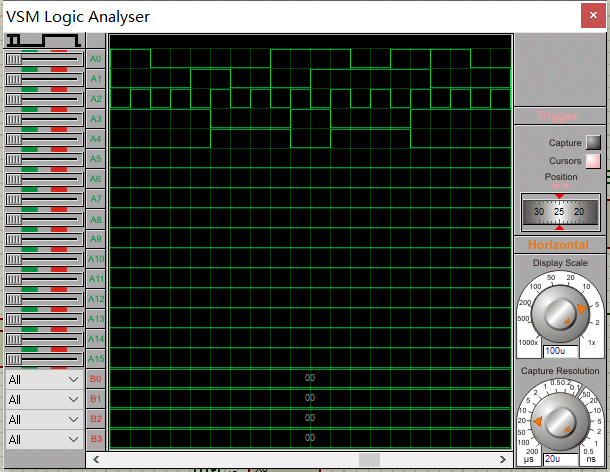
\includegraphics[width=0.8\textwidth]{ex9.8波形图.png}
\end{figure}
图中:分别为J,K,CLK,Q,Q',上升沿有效,JK=10时置位,JK=00时保持,JK=01时清零,JK=00时保持,JK=10时置位,JK=11时翻转,JK=01时清零,JK=11时翻转。
\section{T触发器实现}
\subsection{电路图}
\begin{figure}[H]
    \centering
    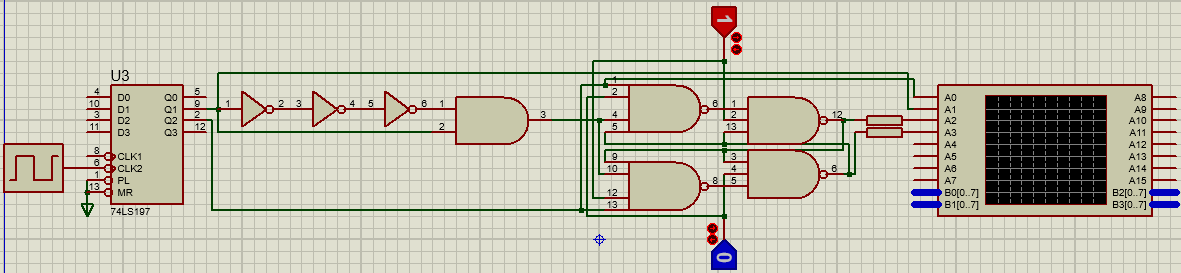
\includegraphics[width=0.8\textwidth]{ex9.9电路图.png}
\end{figure}
\subsection{波形图}
\begin{figure}[H]
    \centering
    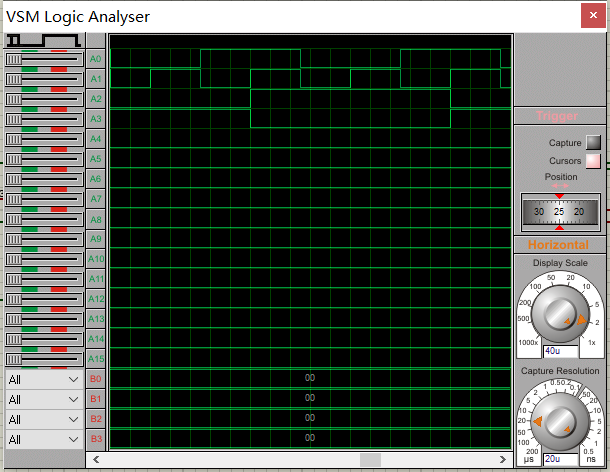
\includegraphics[width=0.8\textwidth]{ex9.9波形图.png}
\end{figure}
图中:分别为T,CLK,Q,Q',上升沿有效,T=0时保持,T=1时翻转。
\section{从学号最后一位开始计数的减法器}
\subsection{电路图}
\begin{figure}[H]
    \centering
    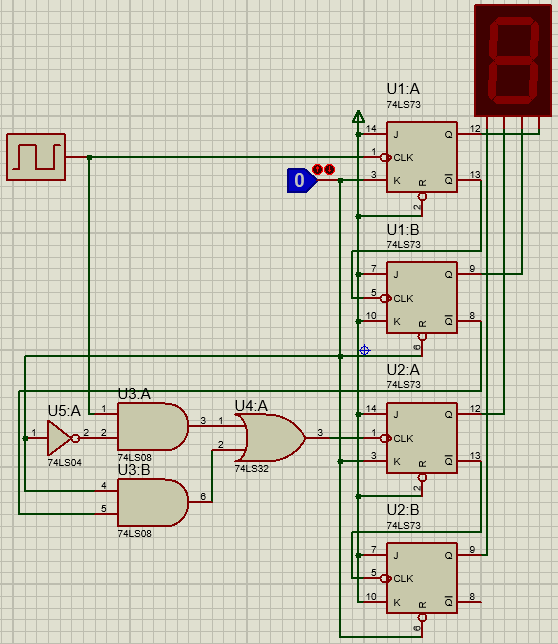
\includegraphics[width=0.8\textwidth]{ex9.10电路图.png}
\end{figure}
如果要初始化为0,则JK接1,R接逻辑电平,如果要初始化为1,则JR接1,K接逻辑电平。
另外初始化1还需要时钟控制,所以在中间的初始化1的触发器,还需要用选择器选择CLK和Qn-1,选择器由逻辑电平控制。
\subsection{视频演示}
\href{run:1.mp4}{点击查看演示视频} 
\section{实验箱实验}
\subsection{J-K触发器动态测试}
\begin{figure}[H]
    \centering
    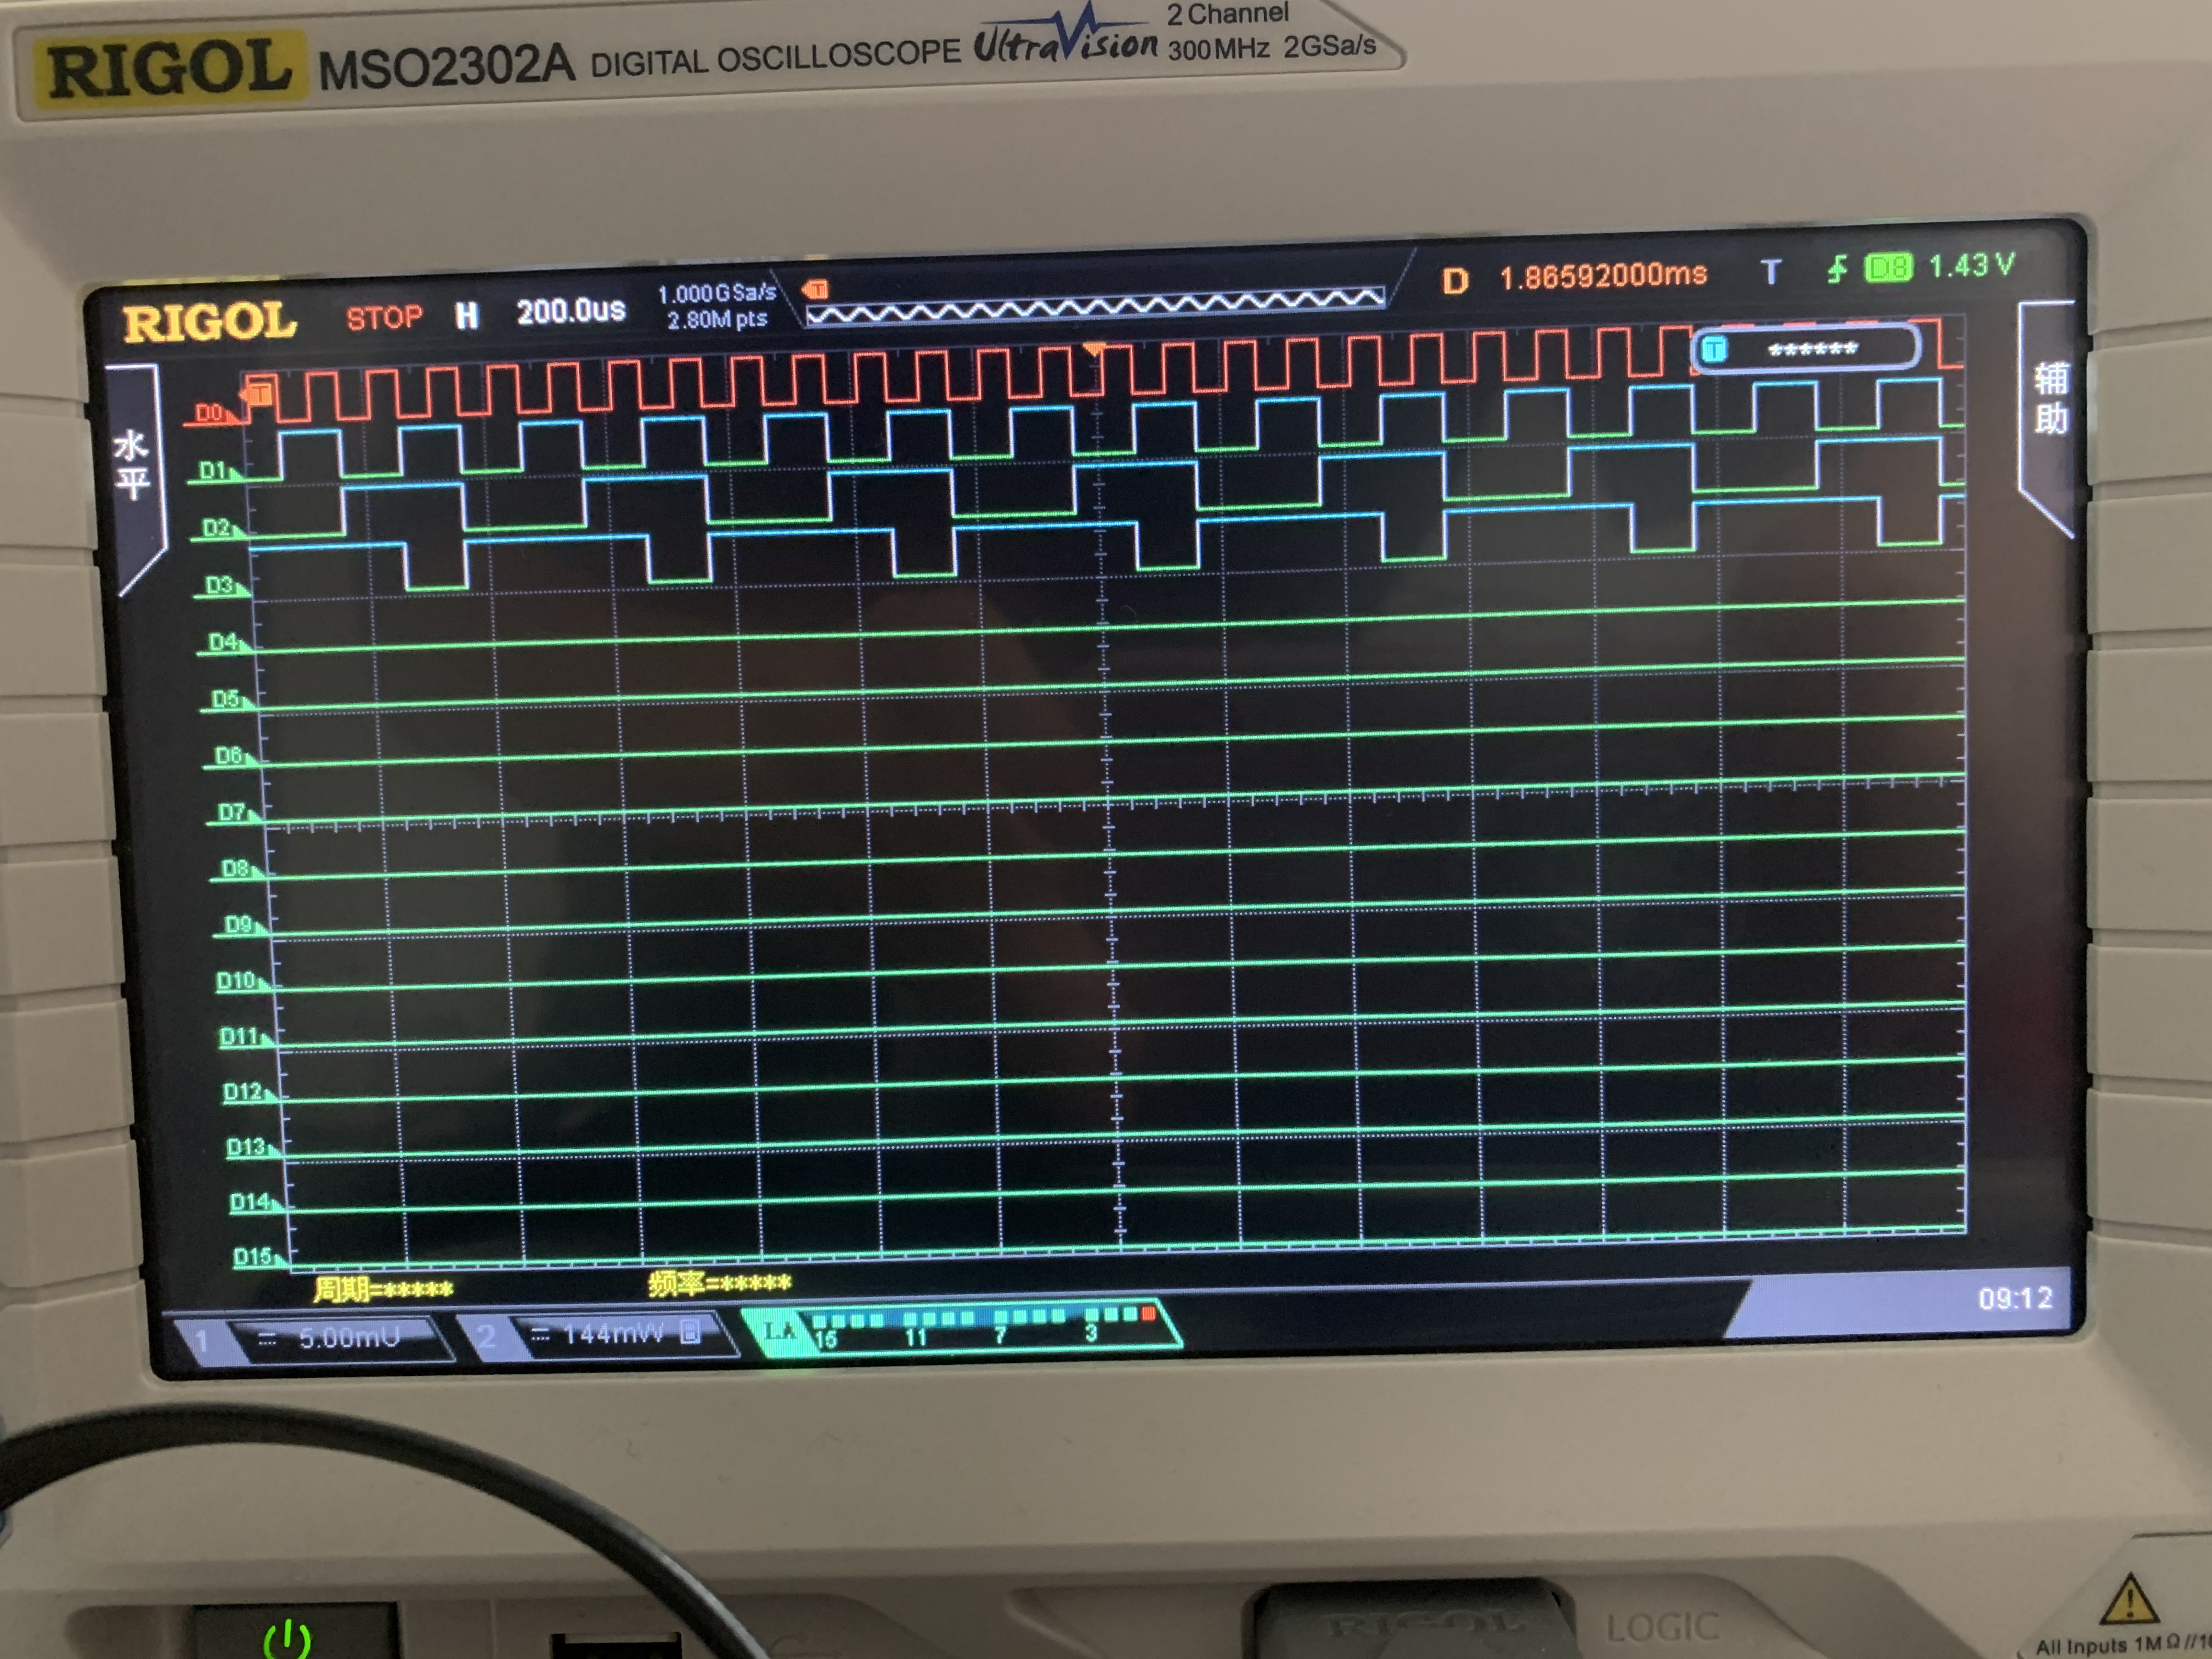
\includegraphics[width=0.8\textwidth]{JK.png}
\end{figure}
\subsection{D触发器动态测试}
\begin{figure}[H]
    \centering
    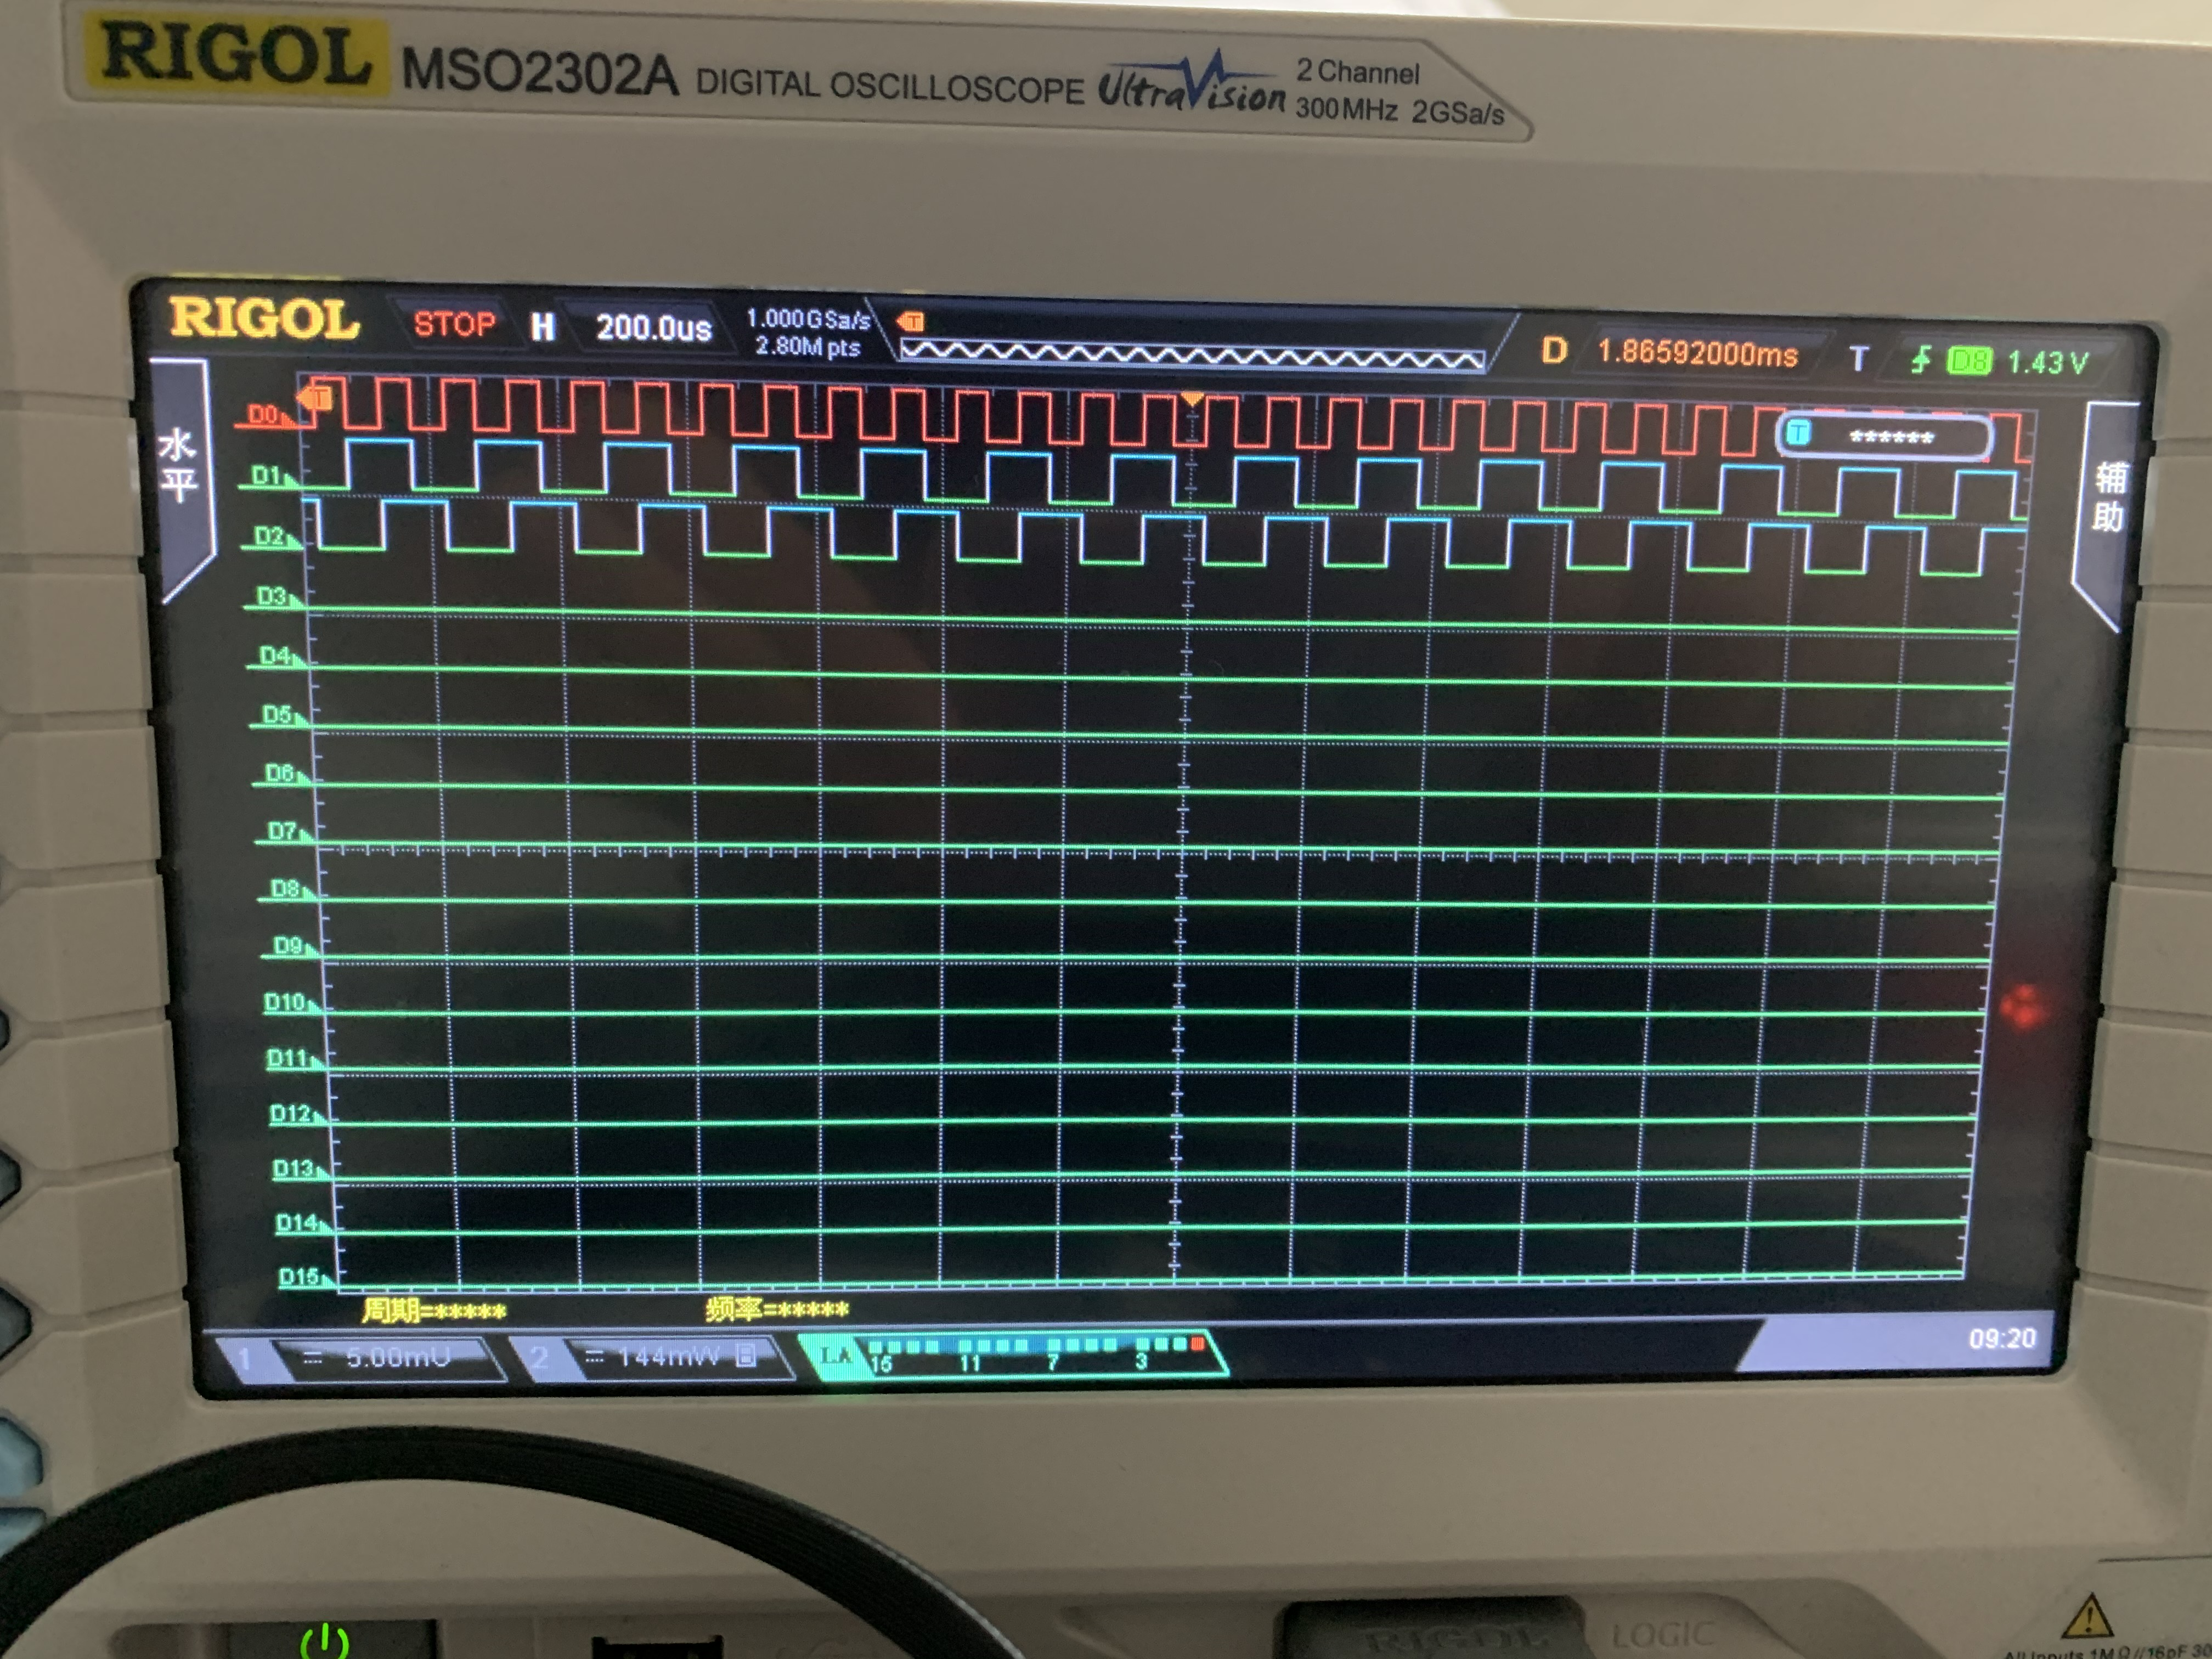
\includegraphics[width=0.8\textwidth]{D.png}
\end{figure}
\subsection{J-K触发器实现D触发器}
\begin{figure}[H]
    \centering
    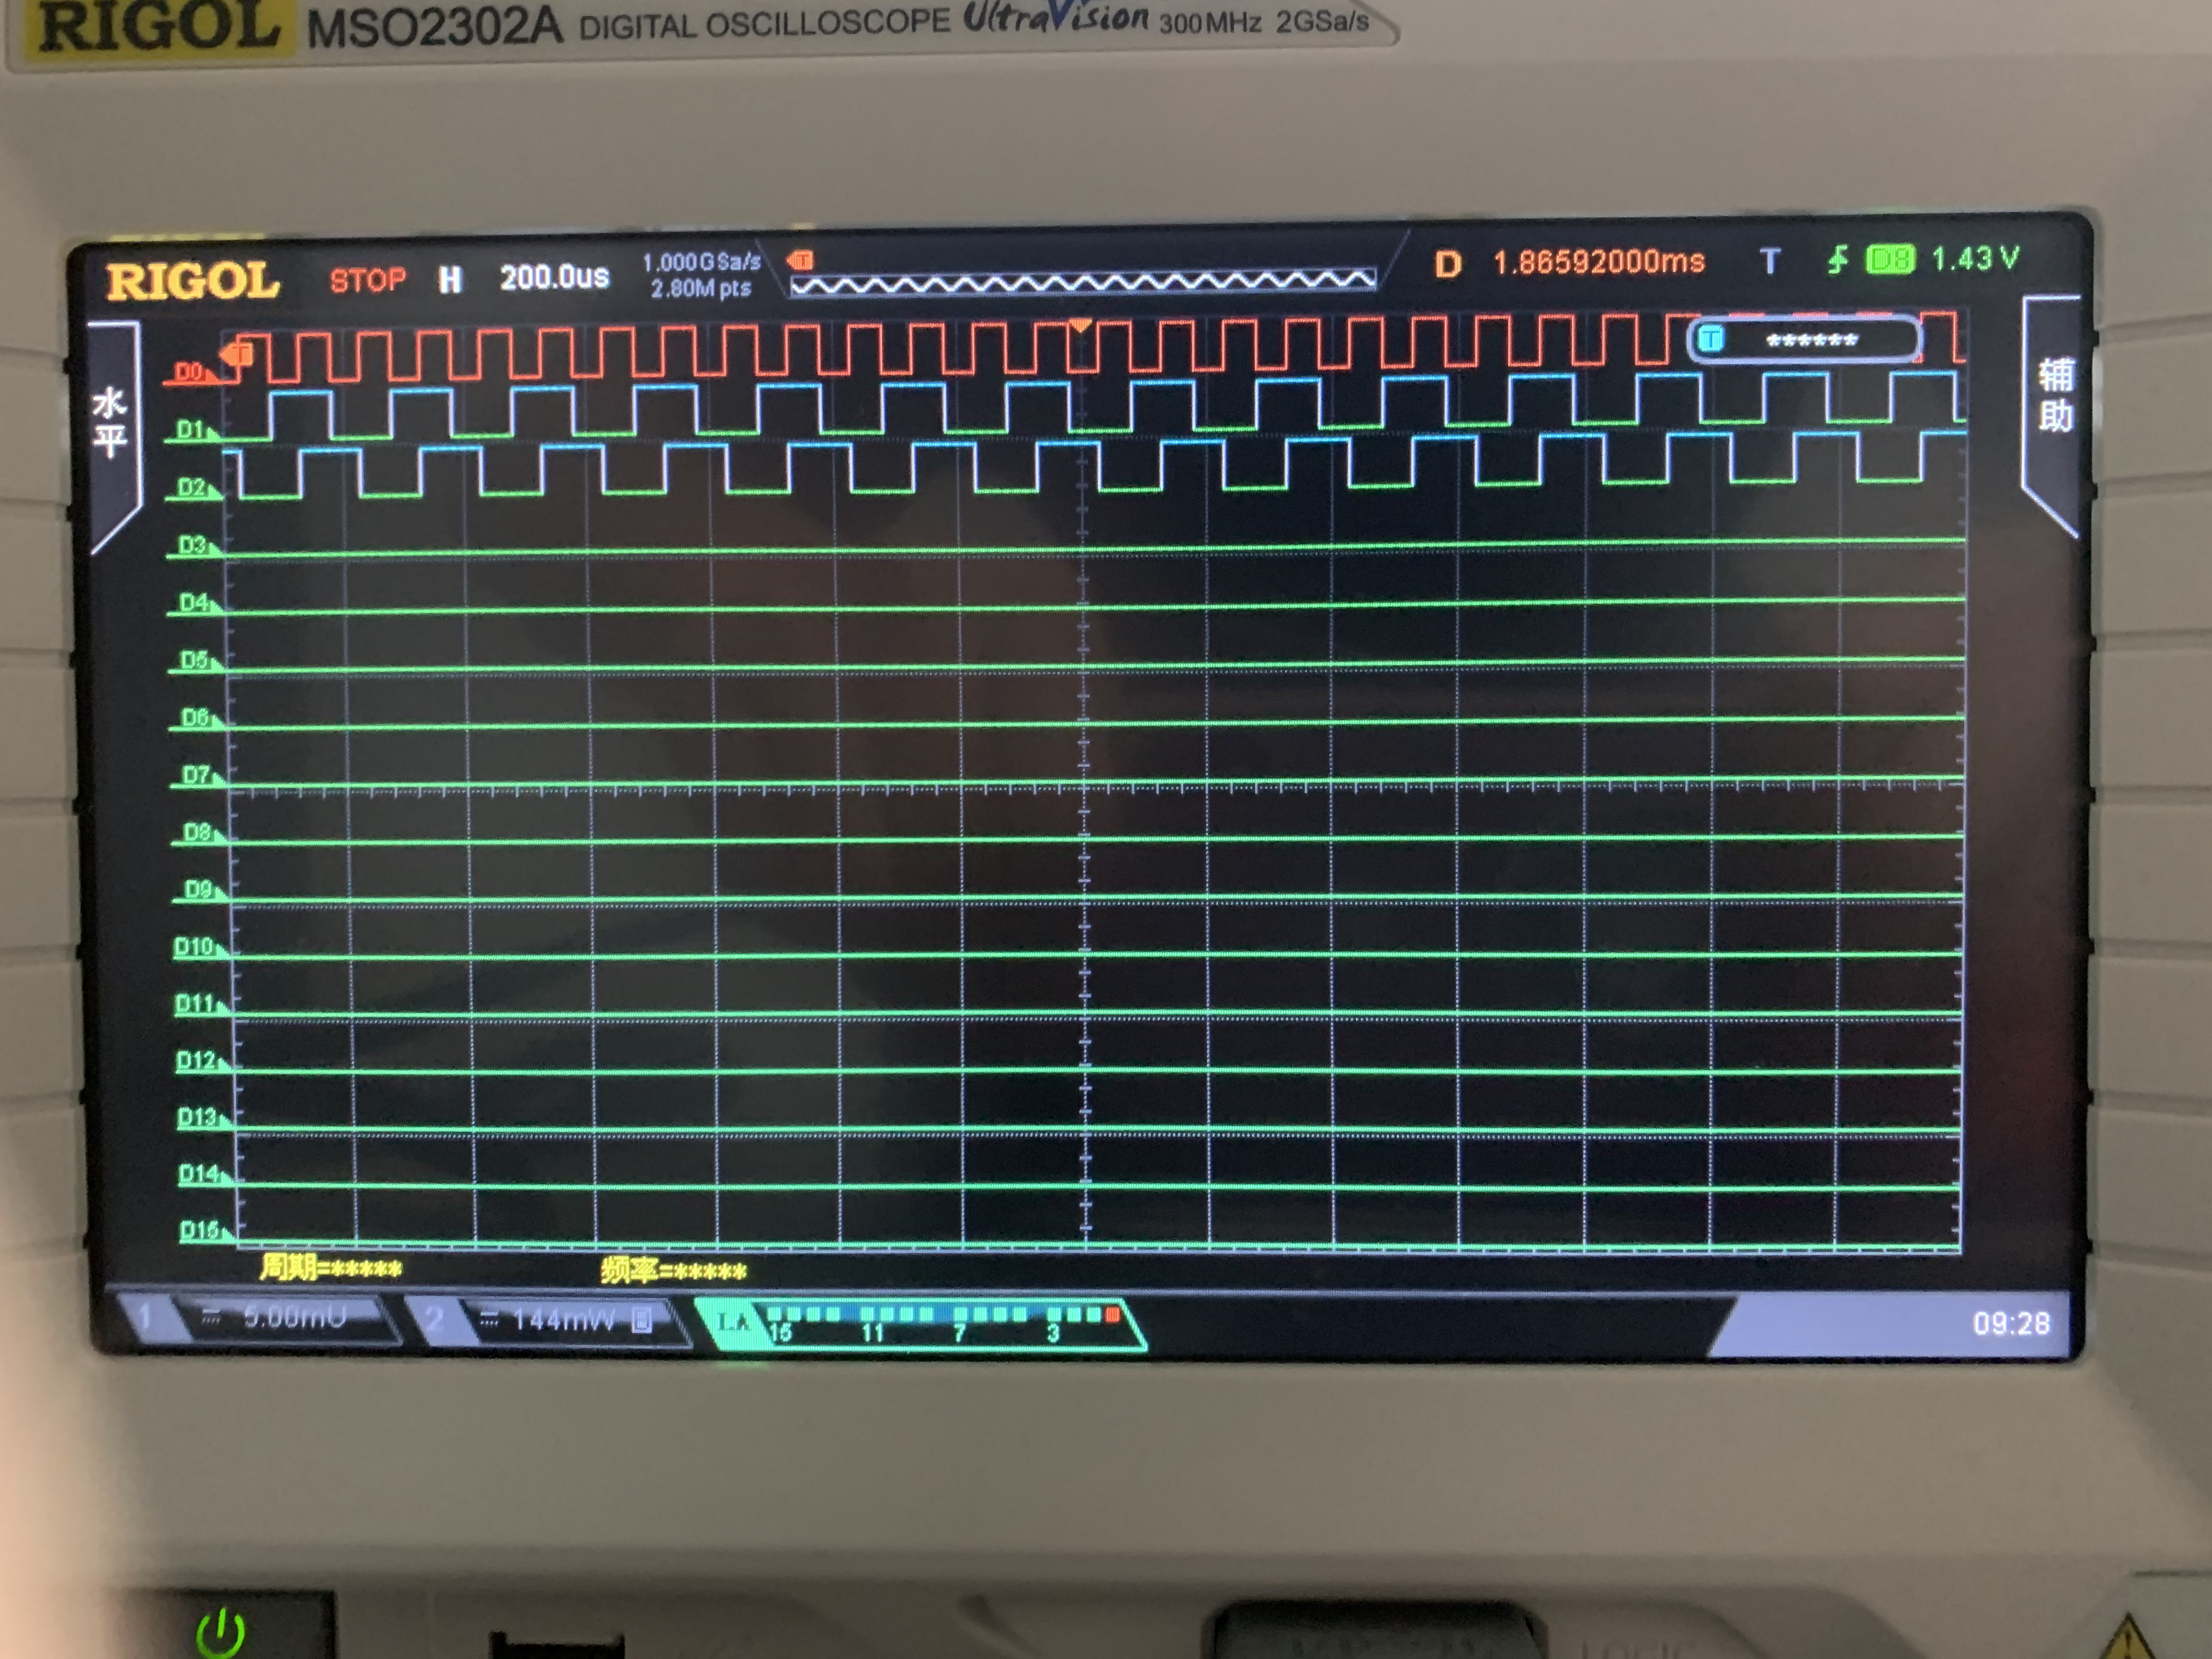
\includegraphics[width=0.8\textwidth]{JK-D.png}
\end{figure}
\subsection{J-K触发器实现T触发器}
\begin{figure}[H]
    \centering
    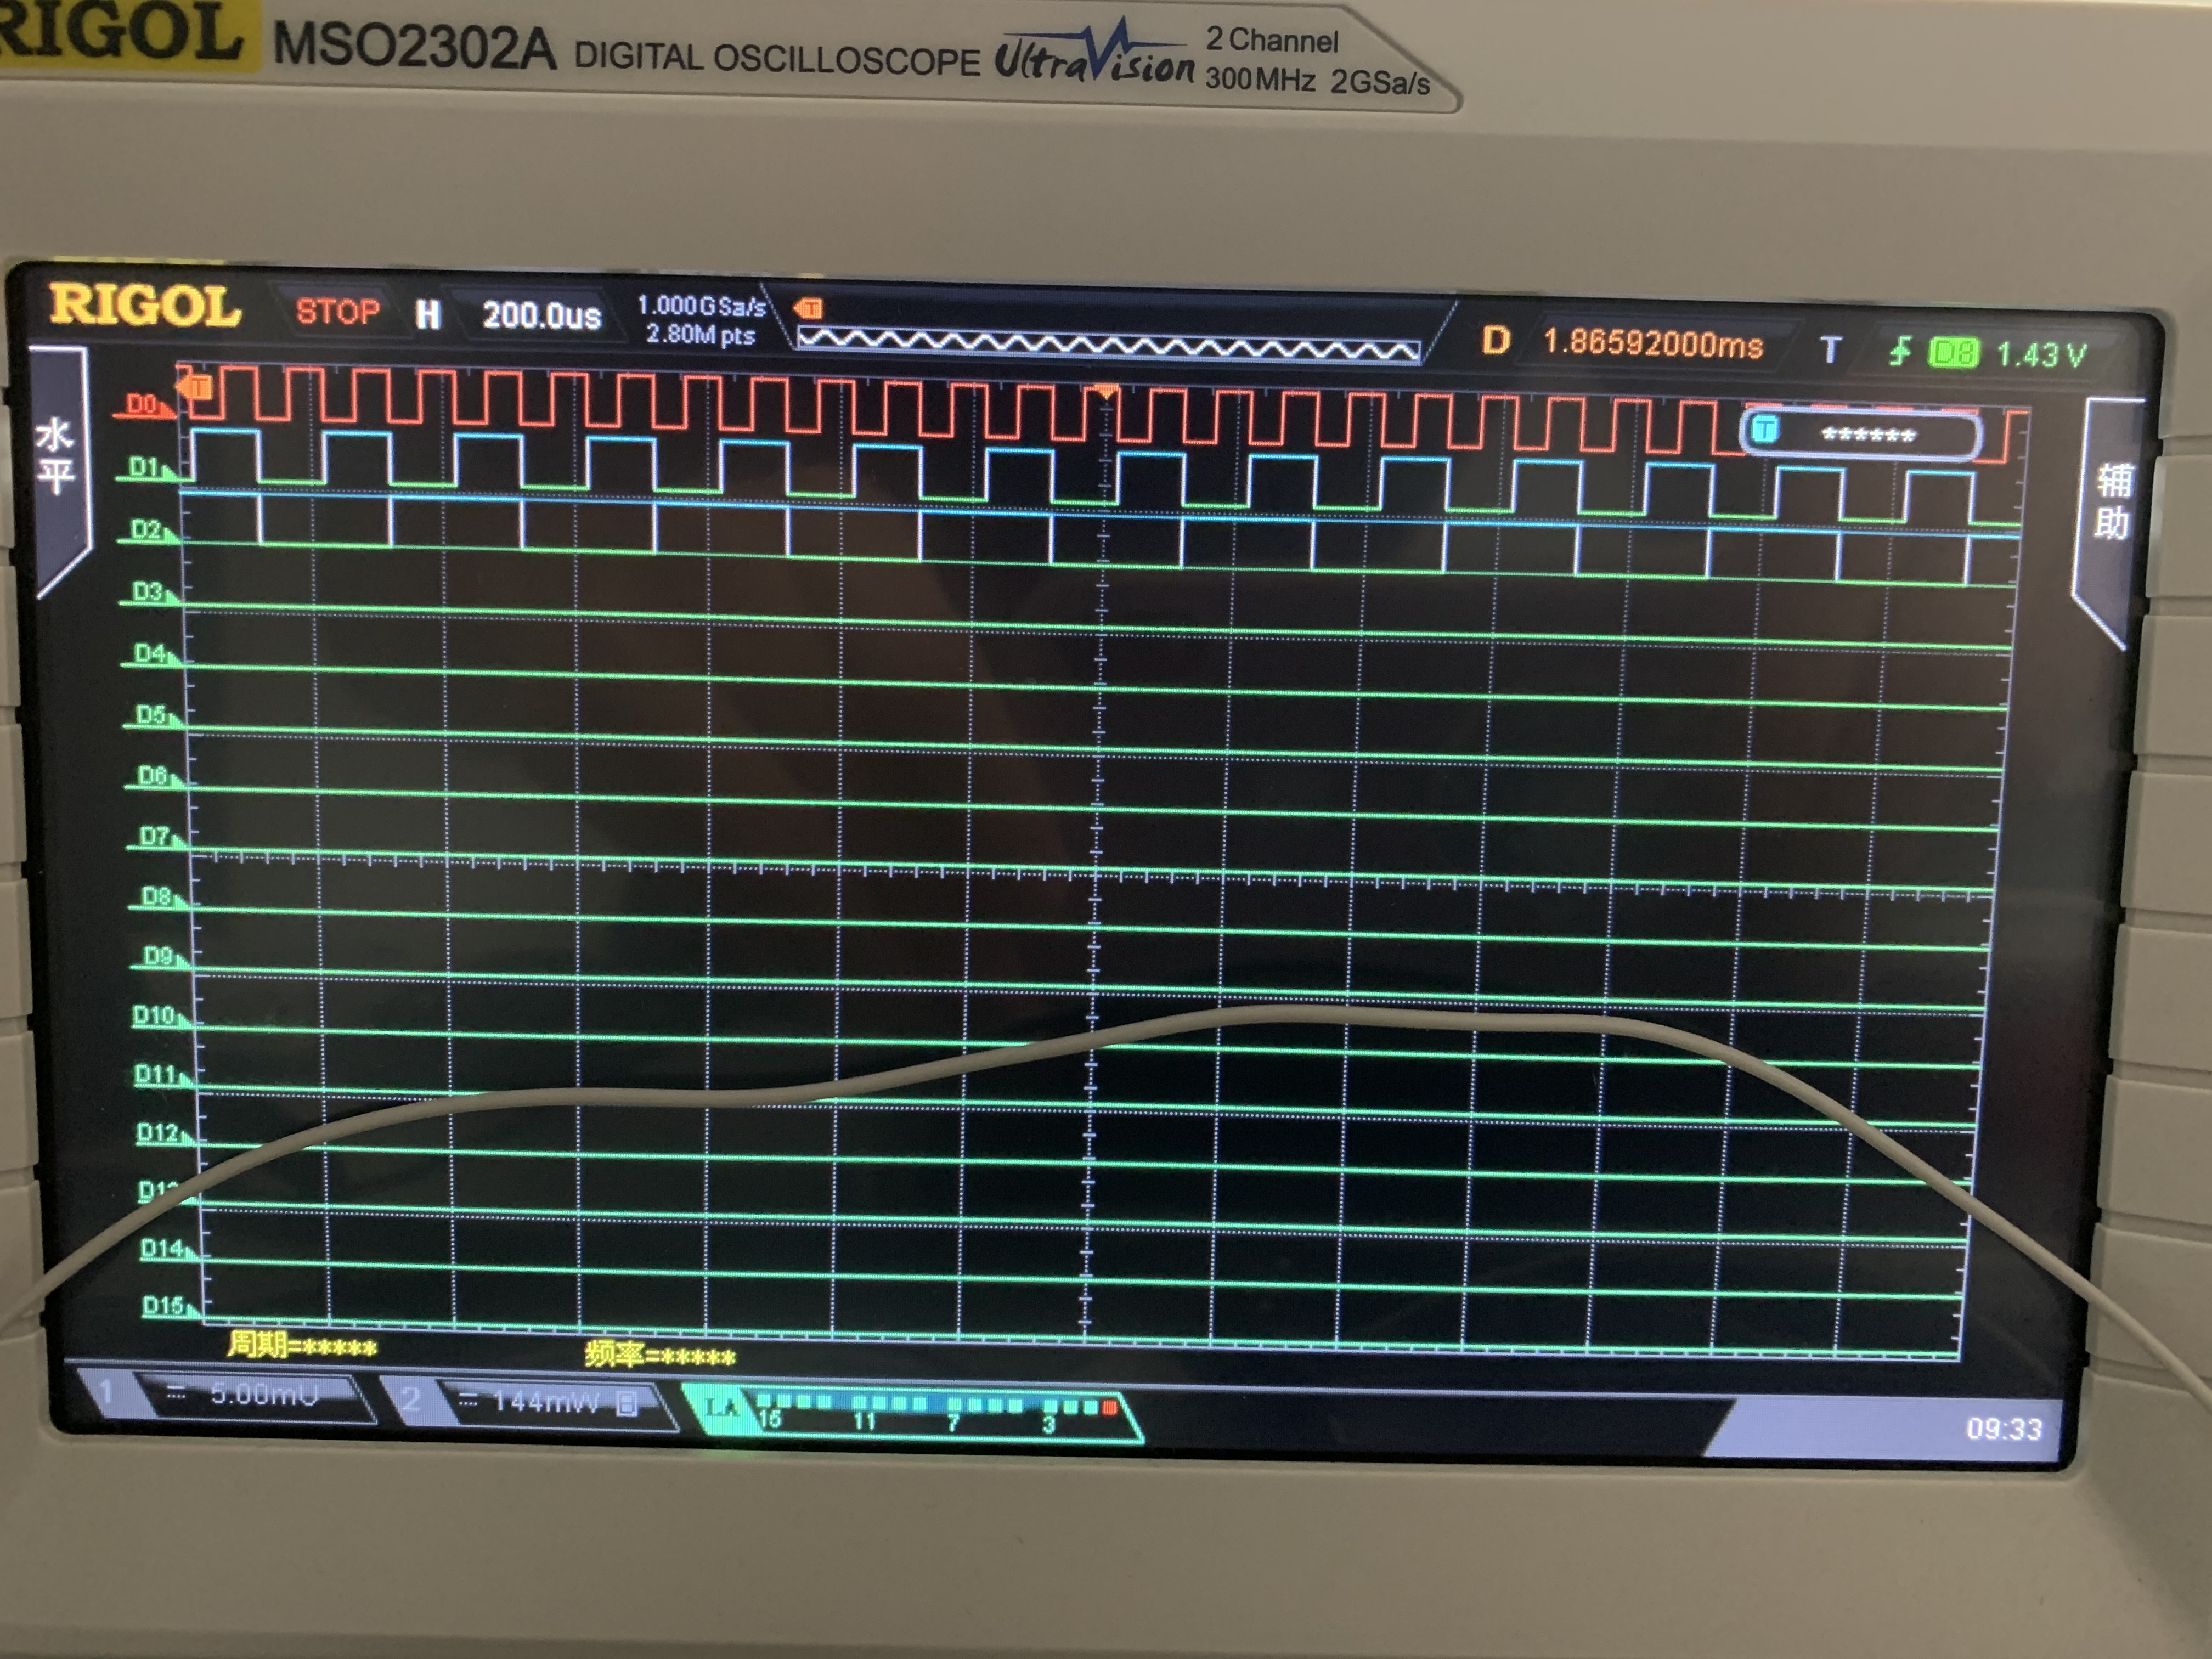
\includegraphics[width=0.8\textwidth]{T.png}
\end{figure}
\section{从学号最后一位开始计数的减法器}
\begin{figure}[H]
    \centering
    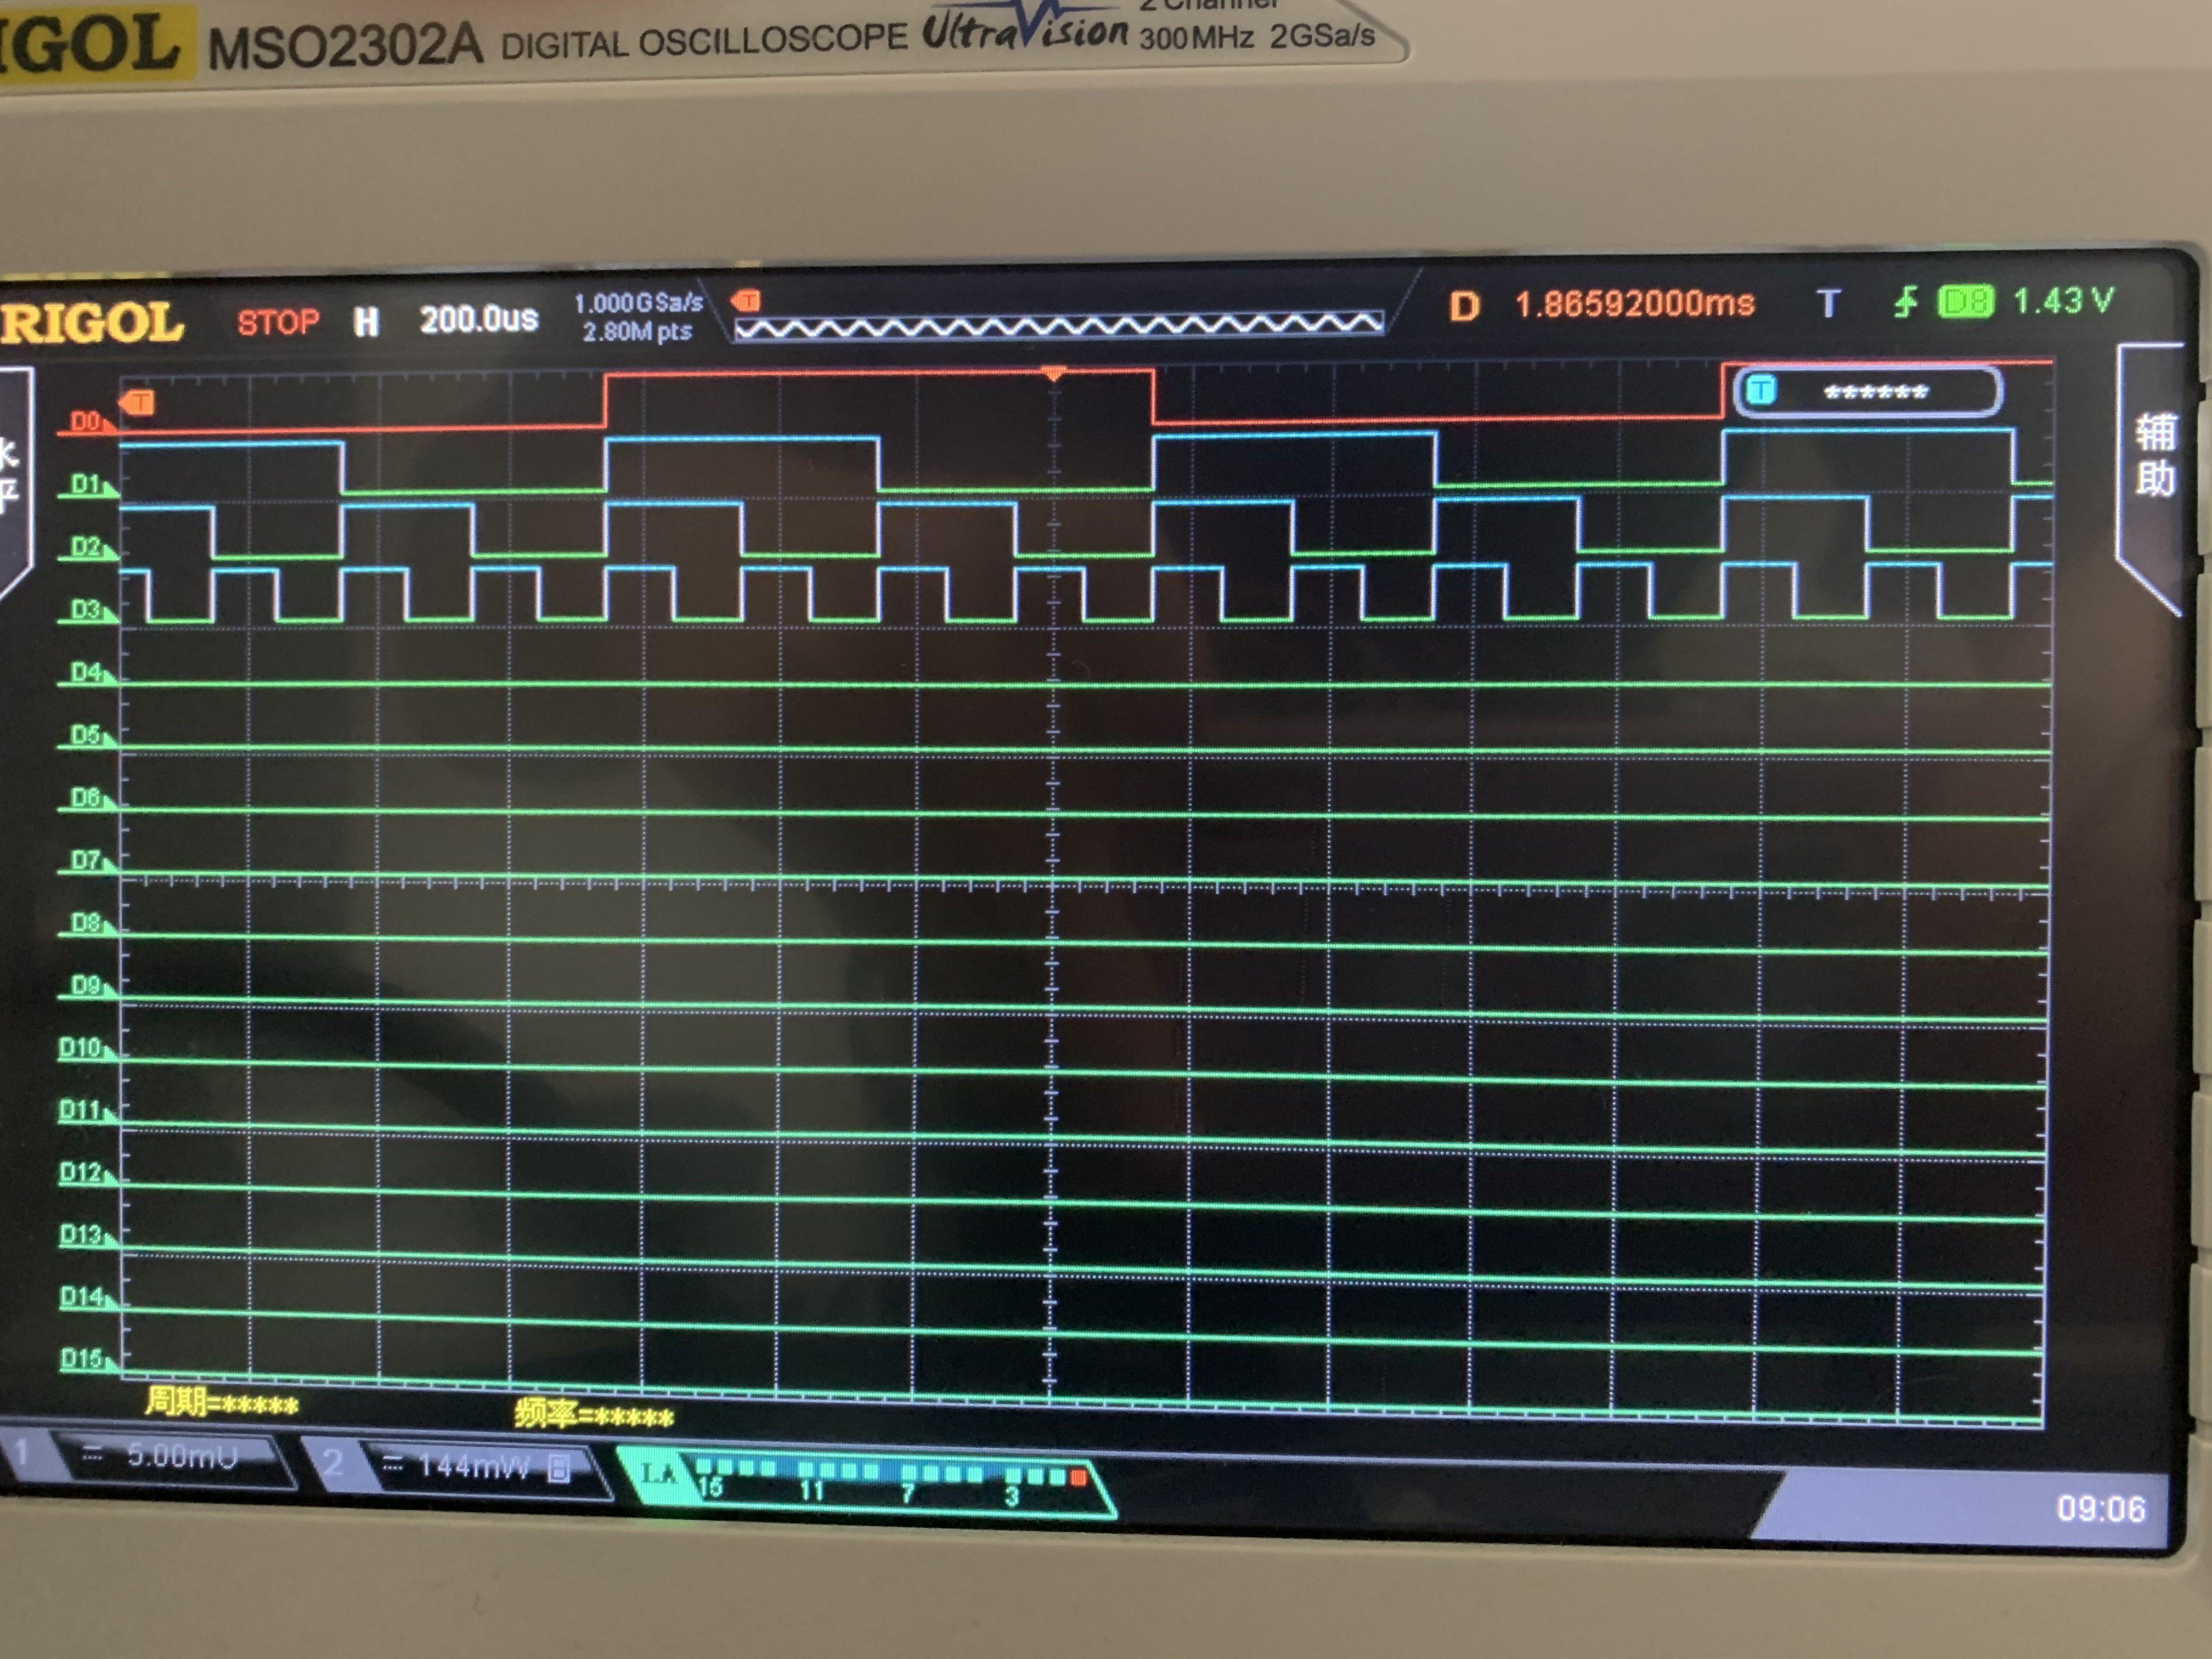
\includegraphics[width=0.8\textwidth]{减法.png}
\end{figure}
\href{run:2.mp4}{点击查看演示视频} 
%\clearpage
%\bibliography{E:/Papers/LiuLab}
%\bibliographystyle{apalike}
\end{document}
%%% Local Variables:
%%% mode: latex
%%% TeX-master: t
%%% End:
